\documentclass{beamer}
\usepackage{amsmath}
\usepackage[english]{babel} %set language; note: after changing this, you need to delete all auxiliary files to recompile
\usepackage[utf8]{inputenc} %define file encoding; latin1 is the other often used option
\usepackage{csquotes} % provides context sensitive quotation facilities
\usepackage{graphicx} %allows for inserting figures
\usepackage{booktabs} % for table formatting without vertical lines
\usepackage{textcomp} % allow for example using the Euro sign with \texteuro
\usepackage{stackengine}
\usepackage{wasysym}
\usepackage{tikzsymbols}
\usepackage{textcomp}
\newcommand{\bubblethis}[2]{
        \tikz[remember picture,baseline]{\node[anchor=base,inner sep=0,outer sep=0]%
        (#1) {\underline{#1}};\node[overlay,cloud callout,callout relative pointer={(0.2cm,-0.7cm)},%
        aspect=2.5,fill=yellow!90] at ($(#1.north)+(-0.5cm,1.6cm)$) {#2};}%
    }%
\tikzset{face/.style={shape=circle,minimum size=4ex,shading=radial,outer sep=0pt,
        inner color=white!50!yellow,outer color= yellow!70!orange}}
%% Some commands to make the code easier
\newcommand{\emoticon}[1][]{%
  \node[face,#1] (emoticon) {};
  %% The eyes are fixed.
  \draw[fill=white] (-1ex,0ex) ..controls (-0.5ex,0.2ex)and(0.5ex,0.2ex)..
        (1ex,0.0ex) ..controls ( 1.5ex,1.5ex)and( 0.2ex,1.7ex)..
        (0ex,0.4ex) ..controls (-0.2ex,1.7ex)and(-1.5ex,1.5ex)..
        (-1ex,0ex)--cycle;}
\newcommand{\pupils}{
  %% standard pupils
  \fill[shift={(0.5ex,0.5ex)},rotate=80] 
       (0,0) ellipse (0.3ex and 0.15ex);
  \fill[shift={(-0.5ex,0.5ex)},rotate=100] 
       (0,0) ellipse (0.3ex and 0.15ex);}

\newcommand{\emoticonname}[1]{
  \node[below=1ex of emoticon,font=\footnotesize,
        minimum width=4cm]{#1};}
\usepackage{scalerel}
\usetikzlibrary{positioning}
\usepackage{xcolor,amssymb}
\newcommand\dangersignb[1][2ex]{%
  \scaleto{\stackengine{0.3pt}{\scalebox{1.1}[.9]{%
  \color{red}$\blacktriangle$}}{\tiny\bfseries !}{O}{c}{F}{F}{L}}{#1}%
}
\newcommand\dangersignw[1][2ex]{%
  \scaleto{\stackengine{0.3pt}{\scalebox{1.1}[.9]{%
  \color{red}$\blacktriangle$}}{\color{white}\tiny\bfseries !}{O}{c}{F}{F}{L}}{#1}%
}
\usepackage{fontawesome} % Social Icons
\usepackage{epstopdf} % allow embedding eps-figures
\usepackage{tikz} % allows drawing figures
\usepackage{amsmath,amssymb,amsthm} %advanced math facilities
\usepackage{lmodern} %uses font that support italic and bold at the same time
\usepackage{hyperref}
\usepackage{tikz}
\hypersetup{
    colorlinks=true,
    linkcolor=blue,
    filecolor=magenta,      
    urlcolor=blue,
}
\usepackage{tcolorbox}
%add citation management using BibLaTeX
\usepackage[citestyle=authoryear-comp, %define style for citations
    bibstyle=authoryear-comp, %define style for bibliography
    maxbibnames=10, %maximum number of authors displayed in bibliography
    minbibnames=1, %minimum number of authors displayed in bibliography
    maxcitenames=3, %maximum number of authors displayed in citations before using et al.
    minnames=1, %maximum number of authors displayed in citations before using et al.
    datezeros=false, % do not print dates with leading zeros
    date=long, %use long formats for dates
    isbn=false,% show no ISBNs in bibliography (applies only if not a mandatory field)
    url=false,% show no urls in bibliography (applies only if not a mandatory field)
    doi=false, % show no dois in bibliography (applies only if not a mandatory field)
    eprint=false, %show no eprint-field in bibliography (applies only if not a mandatory field)
    backend=biber %use biber as the backend; backend=bibtex is less powerful, but easier to install
    ]{biblatex}
\addbibresource{../mybibfile.bib} %define bib-file located one folder higher


\usefonttheme[onlymath]{serif} %set math font to serif ones

\definecolor{beamerblue}{rgb}{0.2,0.2,0.7} %define beamerblue color for later use

%%% defines highlight command to set text blue
\newcommand{\highlight}[1]{{\color{blue}{#1}}}


%%%%%%% commands defining backup slides so that frame numbering is correct

\newcommand{\backupbegin}{
   \newcounter{framenumberappendix}
   \setcounter{framenumberappendix}{\value{framenumber}}
}
\newcommand{\backupend}{
   \addtocounter{framenumberappendix}{-\value{framenumber}}
   \addtocounter{framenumber}{\value{framenumberappendix}}
}

%%%% end of defining backup slides

%Specify figure caption, see also http://tex.stackexchange.com/questions/155738/caption-package-not-working-with-beamer
\setbeamertemplate{caption}{\insertcaption} %redefines caption to remove label "Figure".
%\setbeamerfont{caption}{size=\scriptsize,shape=\itshape,series=\bfseries} %sets figure  caption bold and italic and makes it smaller


\usetheme{Boadilla}

%set options of hyperref package
\hypersetup{
    bookmarksnumbered=true, %put section numbers in bookmarks
    naturalnames=true, %use LATEX-computed names for links
    citebordercolor={1 1 1}, %color of border around cites, here: white, i.e. invisible
    linkbordercolor={1 1 1}, %color of border around links, here: white, i.e. invisible
    colorlinks=true, %color links
    anchorcolor=black, %set color of anchors
    linkcolor=beamerblue, %set link color to beamer blue
    citecolor=blue, %set cite color to beamer blue
    pdfpagemode=UseThumbs, %set default mode of PDF display
    breaklinks=true, %break long links
    pdfstartpage=1 %start at first page
    }


% --------------------
% Overall information
% --------------------
\title[Economía I]{Economía I \vspace{4mm}
\\ Magistral 22: Mercado de crédito}
\date{}
\author[Ertola Navajas y Fariña]{Ertola Navajas y Fariña}
\vspace{0.4cm}
\institute[]{Universidad de San Andrés} 


\begin{document}

\begin{frame}
\titlepage
\centering
Magistral 21


\includegraphics[scale=0.2]{Slides Principios de Economia/Figures/logoUDESA.jpg} 
\end{frame}

\begin{frame}{¿Por qué vamos a estudiar el mercado de crédito?}
    \begin{itemize}
        \item Queremos analizar la voluntad de consumir e invertir de los agentes económicos \vspace{1mm}
        \begin{itemize}
            \item Porque analizar estas dos variables es central para la determinación del consumo y la inversión y, de la demanda agregada
            \item ¿Qué era la demanda agregada? 
        \end{itemize}
        \vspace{3mm}
        \item El mercado de crédito asigna los ahorros de la sociedad a la inversión \vspace{1mm}
        \begin{itemize}
            \item Este mercado representa el mecanismo por el cual la economía reparte la demanda agregada entre consumo e inversión
        \end{itemize}
    \end{itemize}
\end{frame}

\begin{frame}{La Demanda Agregada}
\begin{itemize}
\begin{tcolorbox}[width=4in,
                  interior hidden,
                  boxsep=0pt,
                  left=0pt,
                  right=0pt,
                  top=2pt,
                  ]%%
$$ Y = C + I + G $$
\end{tcolorbox}
    \end{itemize}
\centering donde C + I + G es la absorción.
\vspace{1cm}
\begin{itemize}
        \item \textbf{C} depende de las expectativas, el ingreso disponible e impuestos
        \item \textbf{I} depende de las expectativas, impuestos y productividad
        \item Las dos se ven afectadas por la tasa de interés
        \item Noten que estamos en una economía sin sector externo (no hay exportaciones ni importaciones)
\end{itemize}
\end{frame}

\begin{frame}{¿Cómo se determina el consumo?}
    \begin{itemize}
        \item Depende del ingreso actual y el esperado
        \item La teoría básica del consumo es la de la “suavización del consumo” a lo largo de la vida
        \item Lo que implica que 
            \begin{itemize}
            \item Ante cambios temporarios en el ingreso
                \begin{itemize}
                \item hay pequeños cambios en el consumo (y mucho cambio en el ahorro)
                \end{itemize}            
            \item Ante cambios permanentes en el ingreso
                \begin{itemize}
                \item hay grandes cambios en el consumo actual (y poco cambio en el ahorro)
                \end{itemize}
            \end{itemize}
        \item El consumo cambia más ante cambios en las expectativas que ante cambios reales!!!
        \item Pero la tasa de interés también lo afecta alterando el deseo de "consumo hoy" versus "consumo mañana"
    \end{itemize}
\end{frame}


\begin{frame}{Shocks de ingreso permanentes y transitorios}

\begin{center}
\begin{figure}[h!]
\renewcommand{\figurename}{Figure}
\begin{center}
    \begin{minipage}[b]{0.45\textwidth}
        \begin{center}
\begin{tikzpicture}[scale=0.4]
\draw[very thick,<->] (0,11) node[left]{$C,Y$}--(0,0)--(11,0) node[below]{$t$};

\draw[semithick, gray](0, 4)--(3, 4)--(3,6)--(8.5,6) node[right] {\scriptsize $Y=C$};
\draw[thick, dashed, red](0, 4)--(3, 4)--(3,6)--(8.5,6);
\draw[thick, dotted](3,4)--(3,0) node [below] {\footnotesize $t_0$};
\end{tikzpicture}
\end{center}
     \end{minipage}
  %  \hfill
    \begin{minipage}[b]{0.45\textwidth}
    \begin{center}
\begin{tikzpicture}[scale=0.4]
\draw[very thick,<->] (0,11) node[left]{$C,Y$}--(0,0)--(11,0) node[below]{$t$};
\draw[semithick, gray](0, 4)--(3, 4)--(3,6)--(5,6)--(5,4)--(8.5,4)node[right] {\scriptsize $Y$};
\draw[thick, dashed, red](0, 4)--(3, 4)--(3,5)--(8.5,5) node[right] {\scriptsize $C$};
\draw[thick, dotted](3,4)--(3,0) node [below] {\footnotesize $t_0$};
%\draw[thick, dashed](0, 4)--(3,4)--(3,6)--(5,6);
\end{tikzpicture}
\end{center}
    \end{minipage}
\end{center}
\end{figure}
\end{center}
\end{frame}


\begin{frame}{Shocks de ingreso futuro}
\begin{center}
\begin{figure}[H]
\renewcommand{\figurename}{Figure}
\begin{center}
\begin{tikzpicture}[scale=0.6]
\draw[very thick,<->] (0,11) node[left]{$C,Y$}--(0,0)--(11,0) node[below]{$t$};
\draw[thin, gray](0, 4)--(6, 4)--(6,6)--(8.5,6)node[right] {\scriptsize $Y$};
\draw[thick, dashed, red](0, 4)--(3, 4)--(3,5)--(8.5,5) node[right] {\scriptsize $C$};
\draw[thick, dotted](3,4)--(3,0) node [below] {\footnotesize $t_0$};
\draw[thick, dotted](6,4)--(6,0) node [below] {\footnotesize $t_0+6$};
%\draw[thick, dashed](0, 4)--(3,4)--(3,6)--(5,6);

\end{tikzpicture}
\end{center}
\end{figure}
\end{center}  
\end{frame}


\begin{frame}{Modelo de elección del consumo presente y consumo futuro: la restricción presupuestaria}
    \begin{center}
\begin{figure}[H]
\renewcommand{\figurename}{Figure}
\begin{center}
\begin{tikzpicture}[scale=0.5]
\draw[very thick,<->] (0,11) node[left]{$c_{t+1}$}--(0,0)--(11,0) node[below]{$c_{t}$};
\draw[semithick] (0,7)--(8,0);
 \draw[thick,gray, dashed](3.5, 3.95)--(3.5, 0);
  \draw[thick,gray, dashed](3.5, 3.95)--(0, 3.95);
 \node[below] at (3.5,0) {\footnotesize $y_t$};
  \node[left] at (0,3.95) {\footnotesize $y_{t+1}$};
  \draw[fill] (3.5,3.95) circle [radius =0.11] ;
\end{tikzpicture}
\end{center}
\end{figure}
\end{center} 
\end{frame}


\begin{frame}{Modelo de elección del consumo presente y consumo futuro: la curva de indiferencia}
\begin{center}
\begin{figure}[H]
\renewcommand{\figurename}{Figure}
\begin{center}
\begin{tikzpicture}[scale=0.5]
\draw[very thick,<->] (0,11) node[left]{$c_{t+1}$}--(0,0)--(11,0) node[below]{$c_{t}$};
%\draw[semithick] (2,8).. controls (2.5,2.5) and (4,1) ..(8,0);
\draw[semithick] (2,8).. controls (2.5,2.5) and (4,0.75) ..(8.25,0.65);
 \draw[thick,gray, dashed](2.15, 7)--(2.85, 4);
   \draw[fill] (2.1,7) circle [radius =0.11] ;
 \draw[thick,gray, dashed](4.2, 1.9)--(2.85, 4);      
      \draw[fill] (2.8,3.95) circle [radius =0.11] ;
\draw[fill] (4.2,1.8) circle [radius =0.11] ;      
\draw[semithick, ->] (2.1,7)--(2.1,4);
\draw[semithick, ->] (2.1,3.95)--(2.7,3.95);
\draw[semithick, ->] (2.8,3.95)--(2.8,1.8);
\draw[semithick, ->] (2.85,1.8)--(4,1.8);
\end{tikzpicture}
\end{center}
\end{figure}
\end{center}  
\end{frame}

\begin{frame}{Modelo de elección del consumo presente y consumo futuro: el equilibrio}
\begin{center}
\begin{figure}[H]
\renewcommand{\figurename}{Figure}
\begin{center}
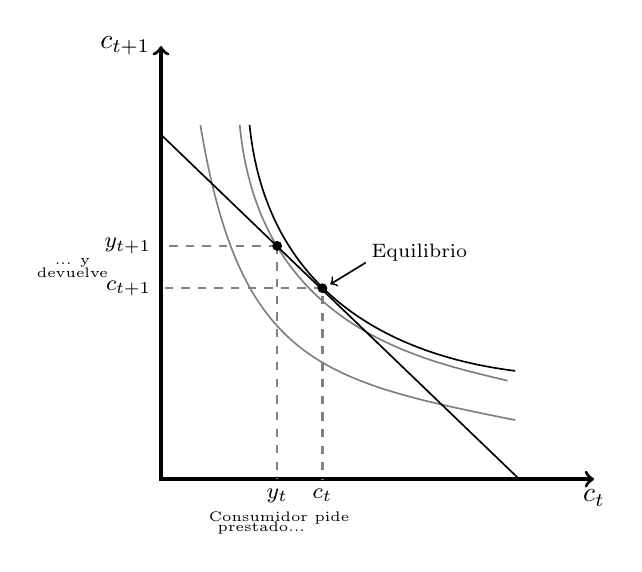
\begin{tikzpicture}[scale=0.5]
\draw[very thick,<->] (0,11) node[left]{$c_{t+1}$}--(0,0)--(11,0) node[below]{$c_{t}$};
\draw[semithick, gray] (1,9).. controls (2,3) and (4, 2.5) .. (9, 1.5) ;
\draw[semithick, gray] (2,9).. controls (2.5,3.75) and (6.8, 3) .. (8.8, 2.5);
\draw[semithick] (2.25,9).. controls (2.75,4) and (7, 3) .. (9, 2.75);
\draw[semithick] (0,8.75)--(9.1,0);
 \draw[thick,gray, dashed](4.1, 4.65)--(4.1, 0);
 \draw[thick,gray, dashed](4.1, 4.85)--(0, 4.85);
 \draw[fill] (4.1,4.85) circle [radius =0.11] ;  
 \node[below] at (4.1,0) {\footnotesize $c_t$};
 \node[left] at (0,4.85){\footnotesize $c_{t+1}$};
 \draw[thick,gray, dashed](2.95, 5.925)--(2.95, 0);
 \draw[thick,gray, dashed](2.95, 5.925)--(0, 5.925);
 \draw[fill] (2.95,5.925) circle [radius =0.11] ;   
 \node[below] at (2.95,0) {\footnotesize $y_t$};
 \node[left] at (0,5.925){\footnotesize $y_{t+1}$};
 \node [right] at (5.1,5.75) {\scriptsize  Equilibrio}  ;
\draw[semithick, <-] (4.3,4.95)--(5.2,5.5);
%\draw [semithick,decorate,decoration={brace,amplitude=3pt,mirror},xshift=5pt,yshift=0pt](2.75,-0.6) -- (3.9,-0.6);
\draw (3,-1) node[]{\tiny Consumidor pide};
\draw (2.55,-1.25) node[]{\tiny prestado...};
%\draw [semithick,decorate,decoration={brace,amplitude=3pt,mirror},xshift=0pt,yshift=5pt](-1.25,5.85) -- (-1.25,4.7);
\draw (-2.25,5.5) node[]{\tiny ... y};
\draw (-2.25,5.25) node[]{\tiny devuelve};
\end{tikzpicture}
\end{center}
\end{figure}
\end{center}  
\end{frame}


\begin{frame}{El efecto de un cambio en la tasa de interés}
\begin{center}
\begin{figure}[H]
\renewcommand{\figurename}{Figure}
\begin{center}
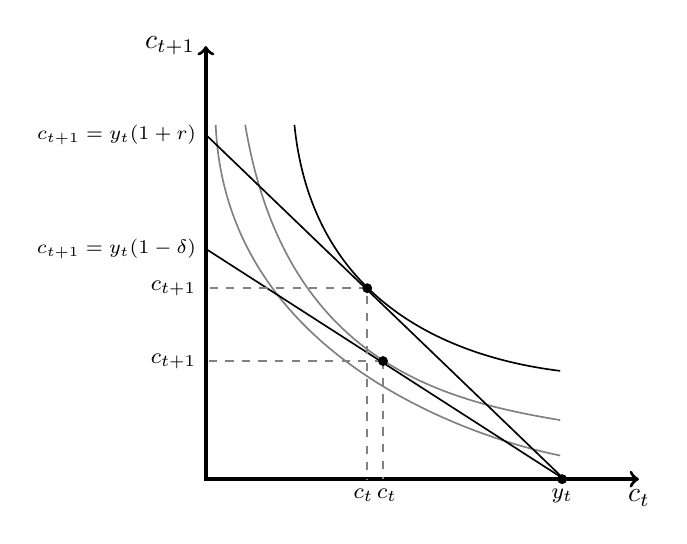
\begin{tikzpicture}[scale=0.5]
\draw[very thick,<->] (0,11) node[left]{$c_{t+1}$}--(0,0)--(11,0) node[below]{$c_{t}$};
\draw[semithick, gray] (1,9).. controls (2,3) and (6, 2) .. (9, 1.5) ;
%\draw[semithick, gray] (0.25,9).. controls (0.5,3) and (7, 1) .. (9, 0);
\draw[semithick, gray] (0.25,9).. controls (0.5,3) and (7, 1) .. (9, 0.6);
\draw[semithick] (2.25,9).. controls (2.75,4) and (7, 3) .. (9, 2.75);
\draw[semithick] (0,8.75)--(9.1,0);
\draw[semithick] (0,5.85)--(9.1,0);
  \draw[thick,gray, dashed](4.1, 4.65)--(4.1, 0);
  \draw[thick,gray, dashed](4.1, 4.85)--(0, 4.85);
  \draw[fill] (4.1,4.85) circle [radius =0.11] ;  
  \node[below] at (4,0) {\footnotesize $c_t$};
  \node[left] at (0,4.85){\footnotesize $c_{t+1}$};
%  \draw[thick,gray, dashed](2.95, 5.925)--(2.95, 0);
%  \draw[thick,gray, dashed](2.95, 5.925)--(0, 5.925);
  \draw[thick,gray, dashed](4.5, 3)--(4.5, 0);
  \draw[thick,gray, dashed](4.5, 3)--(0, 3);
  \node[below] at (4.6,0) {\footnotesize $c_t$};
  \node[left] at (0,3){\footnotesize $c_{t+1}$};
  \draw[fill] (4.5,3) circle [radius =0.11] ;   
    \draw[fill] (9.05,0) circle [radius =0.11] node [below] {\footnotesize $y_t$} ;   
  \node[left] at (0,5.85){\scriptsize $c_{t+1} = y_t (1-\delta)$};   
  \node[left] at (0,8.75){\scriptsize $c_{t+1} = y_t (1+r)$};
\end{tikzpicture}
\end{center}
\end{figure}
\end{center}  
\end{frame}

\begin{frame}{Apalancamiento}
   \begin{center}
\begin{figure}[H]
\renewcommand{\figurename}{Figure}
\begin{center}
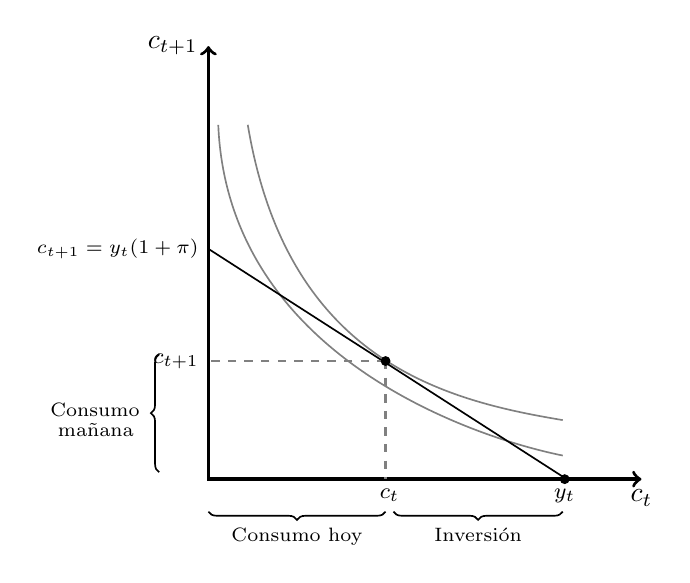
\begin{tikzpicture}[scale=0.5]
\draw[very thick,<->] (0,11) node[left]{$c_{t+1}$}--(0,0)--(11,0) node[below]{$c_{t}$};
\draw[semithick, gray] (1,9).. controls (2,3) and (6, 2) .. (9, 1.5) ;
%\draw[semithick, gray] (0.25,9).. controls (0.5,3) and (7, 1) .. (9, 0);
\draw[semithick, gray] (0.25,9).. controls (0.5,3) and (7, 1) .. (9, 0.6);
\draw[semithick] (0,5.85)--(9.1,0);
  \draw[thick,gray, dashed](4.5, 3)--(4.5, 0);
  \draw[thick,gray, dashed](4.5, 3)--(0, 3);
  \node[below] at (4.6,0) {\footnotesize $c_t$};
  \node[left] at (0,3){\footnotesize $c_{t+1}$};
  \draw[fill] (4.5,3) circle [radius =0.11] ;   
    \draw[fill] (9.05,0) circle [radius =0.11] node [below] {\footnotesize $y_t$} ;   
  \node[left] at (0,5.85){\scriptsize $c_{t+1} = y_t (1+\pi)$};   
 \draw [semithick,decorate,decoration={brace,amplitude=3pt},xshift=0pt,yshift=5pt](-1.25,0) -- (-1.25,3);  
  \draw [semithick,decorate,decoration={brace,amplitude=3pt, mirror},xshift=0pt,yshift=5pt](0,-1) -- (4.5,-1); 
  
    \draw [semithick,decorate,decoration={brace,amplitude=3pt, mirror},xshift=0pt,yshift=5pt](4.7,-1) -- (9,-1); 
  \node[left] at (-1.5,1.75){\scriptsize Consumo};   
    \node[left] at (-1.65,1.25){\scriptsize mañana};
  \node[below] at (2.25,-1){\scriptsize Consumo hoy};      
    \node[below] at (6.85,-1){\scriptsize Inversión};     
\end{tikzpicture}
\end{center}
\end{figure}
\end{center}   
\end{frame}


\begin{frame}{Apalancamiento}
    \begin{center}
\begin{figure}[H]
\renewcommand{\figurename}{Figure}
\begin{center}
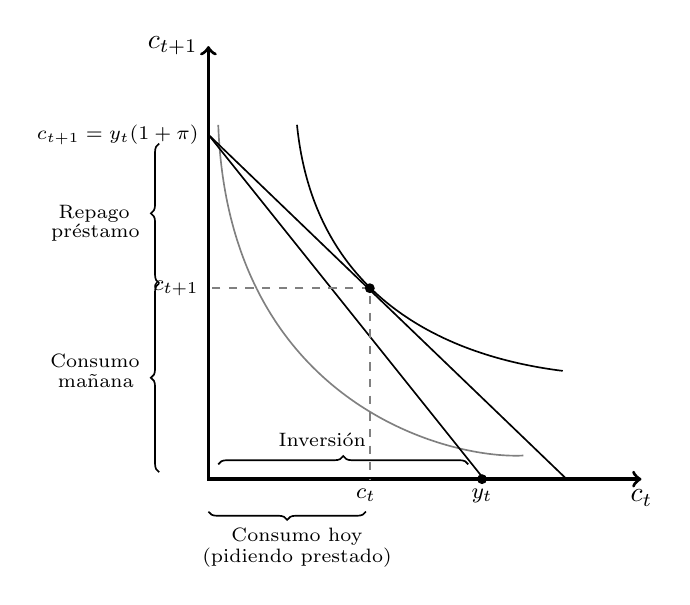
\begin{tikzpicture}[scale=0.5]
\draw[very thick,<->] (0,11) node[left]{$c_{t+1}$}--(0,0)--(11,0) node[below]{$c_{t}$};
%\draw[semithick, gray] (0.25,9).. controls (0.5,2) and (6, 0.5) .. (7, 0);
\draw[semithick, gray] (0.25,9).. controls (0.5,2) and (6, 0.5) .. (8, 0.6);
\draw[semithick] (2.25,9).. controls (2.75,4) and (7, 3) .. (9, 2.75);
\draw[semithick] (0,8.75)--(9.1,0);
\draw[semithick] (0,8.75)--(7,0);
  \draw[thick,gray, dashed](4.1, 4.65)--(4.1, 0);
  \draw[thick,gray, dashed](4.1, 4.85)--(0, 4.85);
  \draw[fill] (4.1,4.85) circle [radius =0.11] ;  
  \node[below] at (4,0) {\footnotesize $c_t$};
  \node[left] at (0,4.85){\footnotesize $c_{t+1}$};
    \draw[fill] (6.95,0) circle [radius =0.11] node [below] {\footnotesize $y_t$} ;   
  \node[left] at (0,8.75){\scriptsize $c_{t+1} = y_t (1+\pi)$}; 
   \draw [semithick,decorate,decoration={brace,amplitude=3pt},xshift=0pt,yshift=5pt](-1.25,0) -- (-1.25,4.8); 
      \draw [semithick,decorate,decoration={brace,amplitude=3pt,mirror},xshift=0pt,yshift=5pt](-1.25,8.35) -- (-1.25,4.8); 
  \draw [semithick,decorate,decoration={brace,amplitude=3pt, mirror},xshift=0pt,yshift=5pt](0,-1) -- (4,-1); 
\draw [semithick,decorate,decoration={brace,amplitude=3pt},xshift=0pt,yshift=5pt](0.25,0.2) -- (6.6,0.2); 
  \node[left] at (-1.5,3){\scriptsize Consumo};   
    \node[left] at (-1.65,2.5){\scriptsize mañana};
  \node[below] at (2.25,-1){\scriptsize Consumo hoy};
  \node[below] at (2.25,-1.5){\scriptsize (pidiendo prestado)};
    \node[left] at (4.25,1){\scriptsize Inversión};
      \node[left] at (-1.75,6.75){\scriptsize Repago };   
    \node[left] at (-1.5,6.25){\scriptsize préstamo};
\end{tikzpicture}
\end{center}
\end{figure}
\end{center} 
\end{frame}

\begin{frame}{El Gran Elon}
   \begin{figure} [H]
    \centering
    \href{https://twitter.com/Stelladmarco/status/1103059259586052097}{
    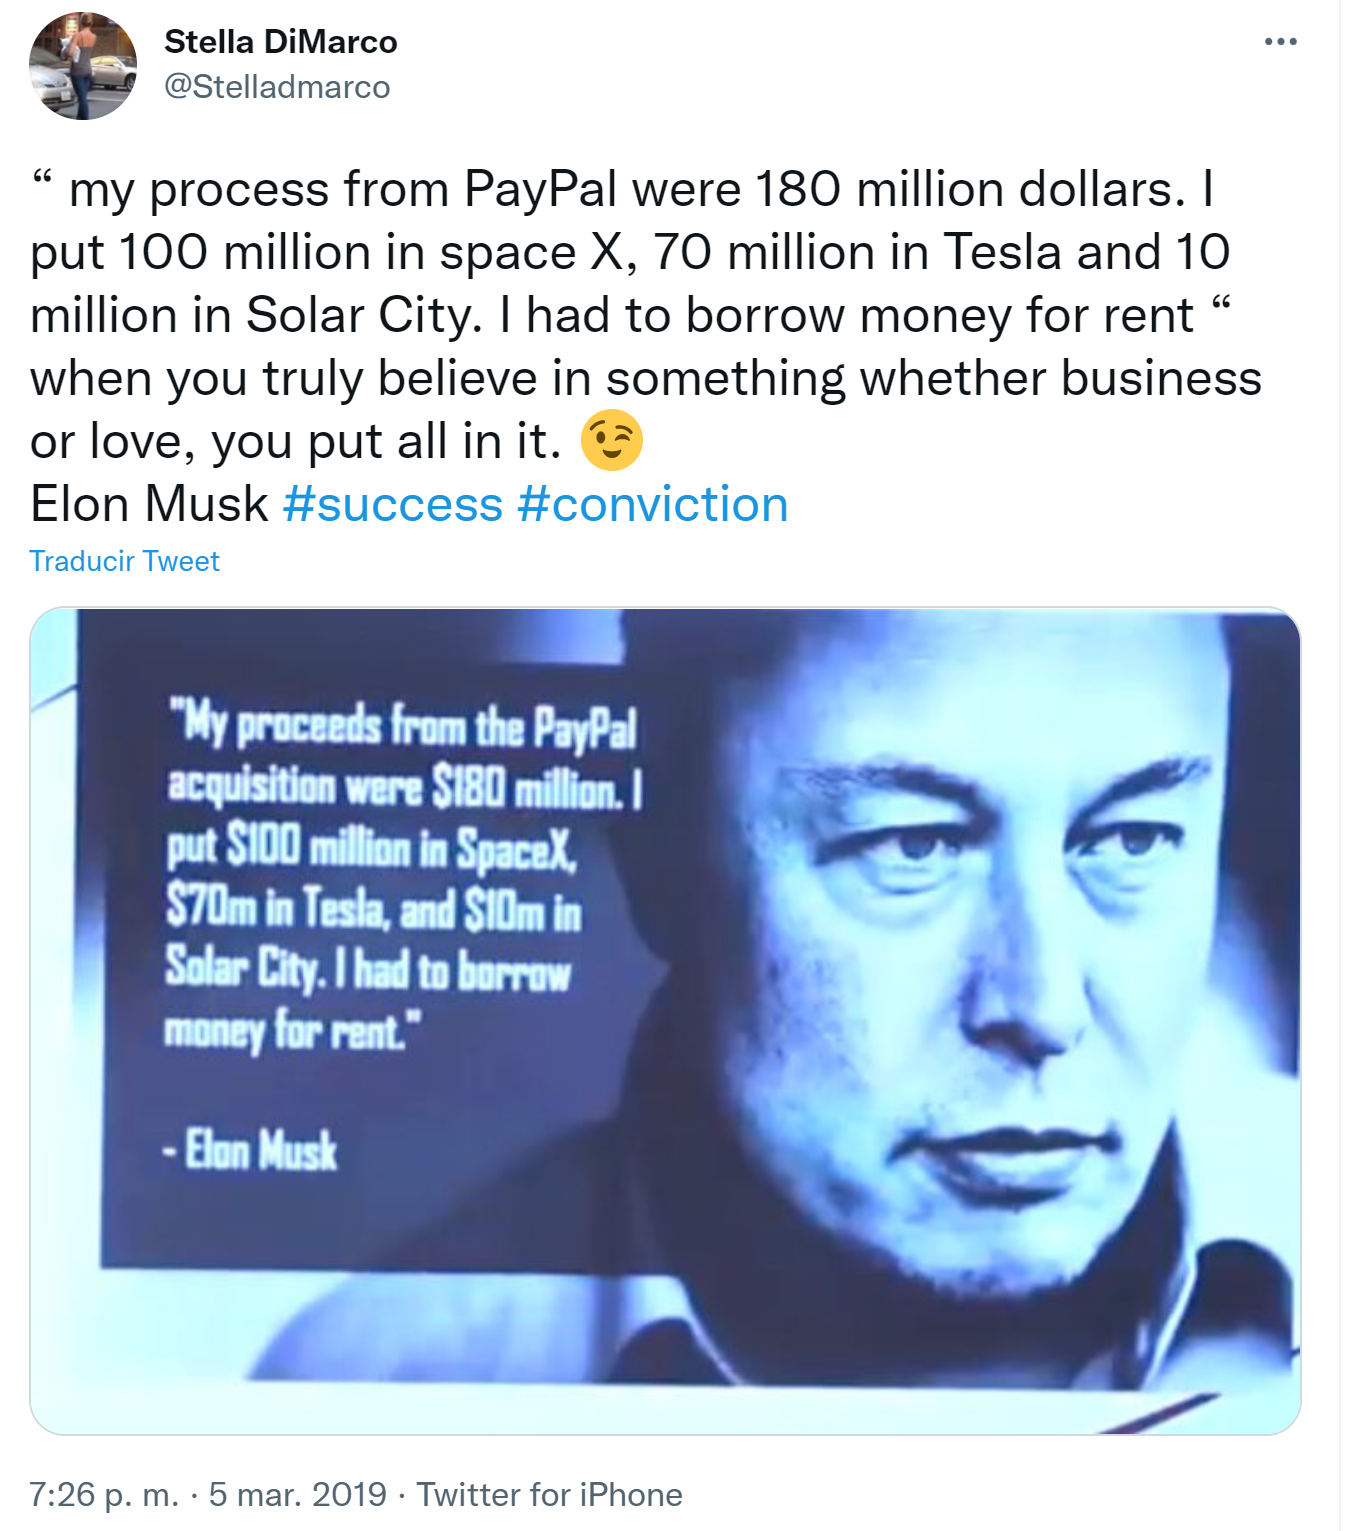
\includegraphics[scale=0.5]{Slides Principios de Economia/Figures/C31.9.png}}
\end{figure} 
\end{frame} 


\begin{frame}{Otras teorías del ahorro}
   \begin{itemize}
       \item Ciclo de vida
       \item Hipotecas revertidas
       \item Los tests de Shea
       \item Ahorro precautorio
       \item La fuerza de los defaults
       \item Present bias
       \item Ubank
   \end{itemize} 
\end{frame}


\begin{frame}{La inversión: valor presente}
    \begin{equation}
VPN = \sum_{t=0} ^{T} \frac{1}{(1+r)^t} W_t,
\end{equation}
\begin{itemize}
    \item $r$ es el costo del capital 
    \item Si el VPN$>0$, entonces convendría invertir
    \item Si VPN $<0$ no convendría
\end{itemize}
\end{frame}


\begin{frame}{El WACC}
\begin{itemize}
    \item  ¿Cuál es el costo de capital que deberíamos usar?
    \item La manera mas conocida es la del costo capital promedio ponderado (CCPP, o WACC por sus siglas en inglés)
\end{itemize}
     
\begin{equation}
WACC=\alpha _{eq}r_{eq}+\left( 1-\alpha _{eq}\right) r_{debt},
\end{equation}

\begin{equation}
\alpha _{eq}=\left( \frac{\text{Net worth}}{\text{Total Assets}}\right) 
\end{equation}
\end{frame}

\begin{frame}{La opción de invertir de Pindyck}
    Supongamos que podemos hacer una inversión inicial de \$2200, lo que nos lleva al siguiente pago estocástico:
    \begin{center}
\begin{tabular}{cccc}
\begin{array}{cccc}
t=0 & & t=1& \hspace{0.15cm} t=2\\[1.5mm]
& q &P_{1} = 300&\hspace{0.15cm}... \\
P_{0}=200&&&\\
&1-q&P_{1} = 100&\hspace{0.15cm} ...  \\
\end{array}
\end{tabular}
\end{center}
\end{frame}


\begin{frame}{La opción de invertir de Pindyck}
    \begin{equation}
VPN= - 2200+\sum\limits_{t=0}^{\infty }\frac{200}{\left( 1.1\right) ^{t}}%
=-2200+2200=\$0.  \label{basic}
\end{equation}

\end{frame}

\begin{frame}{La opción de invertir de Pindyck}
¿Qué pasa si espero un periodo para invertir?
\scriptsize
\begin{equation}
VPN=0.5\left[ -\frac{2200}{1.1}+\sum\limits_{t=1}^{\infty }\frac{300}{%
\left( 1.1\right) ^{t}}\right] =0.5\left[ -\frac{2200}{1.1}+\frac{300}{%
\left( 1.1\right) }\left( 1+\frac{1}{1.1}+\frac{1}{1.1^{2}}+ ... \right) %
\right]
\end{equation}

\begin{equation}
=0.5\left[ -\frac{2200}{1.1}+\frac{300}{\left( 1.1\right) }\left( \frac{1%
}{1-\frac{1}{1.1}}\right) \right] =0.5\left[ -\frac{2200}{1.1}+\frac{300}{%
\left( 1.1\right) }\left( \frac{1.1}{0.1}\right) \right] = 500!
\end{equation}
\end{frame}

\begin{frame}{Demanda agregada y el mercado de crédito}

    \begin{itemize}
\begin{tcolorbox}[width=4in,
                  interior hidden,
                  boxsep=0pt,
                  left=0pt,
                  right=0pt,
                  top=2pt,
                  ]%%
$$ Y = C(r) + I(r) + G $$
\end{tcolorbox}
    \end{itemize}
    
\centering \small{donde r es la tasa de interés real}

 \begin{itemize}
        \item En una economía cerrada:
        
        \begin{tcolorbox}[width=4in,
                  interior hidden,
                  boxsep=0pt,
                  left=0pt,
                  right=0pt,
                  top=2pt,
                  ]%%
                    $$ Y – C(r) – G(r) = I $$
        \end{tcolorbox}
        
    \end{itemize}
    \begin{itemize}
        \item Que es como decir que lo que ahorro es lo que invierto
        \item Y esto determina la tasa de interés real
        \item Los ahorros son intermediados por el sector financiero hacia inversiones reales
        \item Economías que ahorran mucho invierten mucho (China, Japón), economías que ahorran poco invierten menos (Brasil, Argentina)! 
    \end{itemize}
 \end{frame}


\begin{frame}{El mercado de crédito}
\begin{center}
\begin{figure}[H]
\renewcommand{\figurename}{Figure}
\begin{center}
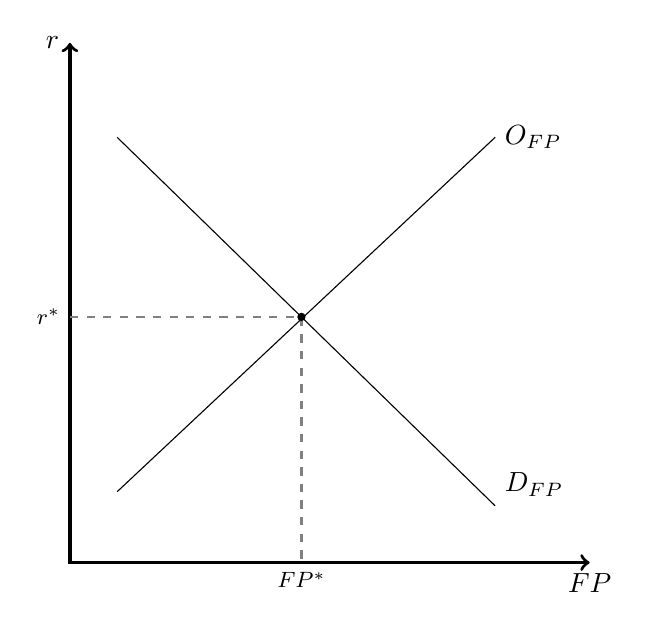
\begin{tikzpicture}[scale=0.6]
\draw[very thick,<->] (0,11) node[left]{$r$}--(0,0)--(11,0) node[below]{$FP$};

%\node[] at(5,-1.5) {\underline{Mercado de Crédito}};
\draw[thin](1,1.5)--(9,9) node [right] {$O_{FP}$};
\draw[thin](1,9)--(9,1.2) node [above right] {$D_{FP}$};
\draw[thick,dashed,gray] (0,5.2)--(4.9,5.2)--(4.9,0);
\draw[fill] (4.9,5.2) circle [radius =0.075]; 
\node[below] at (4.9,0) {\footnotesize $FP^{*}$};
\node[left] at (0,5.2) {\footnotesize $r^{*}$};
\end{tikzpicture}
\end{center}
\end{figure}
\end{center}  
\end{frame}

\begin{frame}{El mercado de crédito}
    \begin{center}
\begin{figure}[H]
\renewcommand{\figurename}{Figure}
\begin{center}
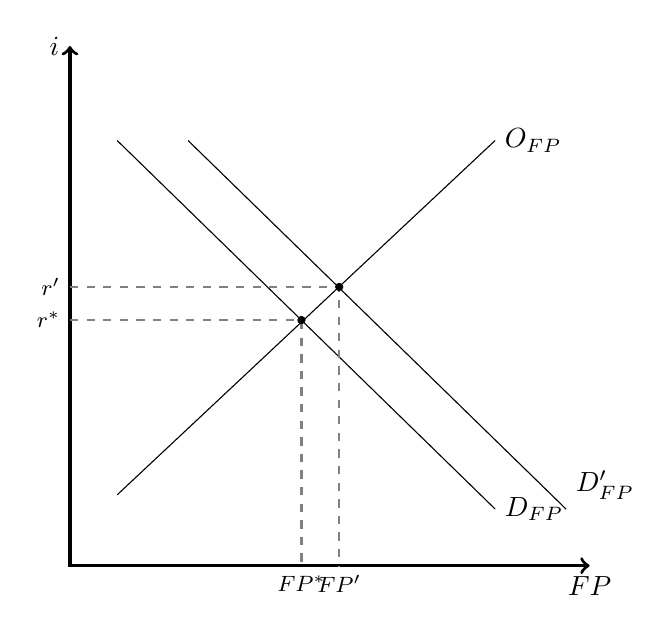
\begin{tikzpicture}[scale=0.6]
\draw[very thick,<->] (0,11) node[left]{$i$}--(0,0)--(11,0) node[below]{$FP$};
\draw[thin](1,1.5)--(9,9) node [right] {$O_{FP}$};
\draw[thin](1,9)--(9,1.2) node [right] {$D_{FP}$};
\draw[thin](2.5,9)--(10.5,1.2) node [above right] {$D_{FP}'$};
\draw[thick,dashed,gray] (0,5.2)--(4.9,5.2)--(4.9,0);
\draw[thick,dashed,gray] (0,5.9)--(5.7,5.9)--(5.7,0);
\draw[fill] (4.9,5.2) circle [radius =0.075]; 
\draw[fill] (5.7,5.9) circle [radius =0.075]; 
\node[below] at (4.9,0) {\footnotesize $FP^{*}$};
\node[left] at (0,5.2) {\footnotesize $r^{*}$};
\node[below] at (5.7,0) {\footnotesize $FP'$};
\node[left] at (0,5.9) {\footnotesize $r'$};
\end{tikzpicture}
\end{center}
\end{figure}
\end{center}  
\end{frame}



\end{document}